\section{\framework Overview}


\framework is a mid-end compiler framework for DSLs. Using this framework, DSLs can transform their architecture-independent intermediate representations to a single-thread-optimizing back-end intermediate representation while taking advantage of modern architectural features  such as multicore parallelism, non-uniform memory (NUMA) hierarchies, clusters, and accelerators like graphics processing units (GPUs).
It is designed mainly for programs that operate over dense data using loop nests.
\subsection{Why Separation is Necessary}

Mid-end compilers need to schedule the iterations onto a modern architecture to take advantage of available parallelism and manage the complex memory hierarchy.
In many cases, it is difficult to know the best data-mapping before deciding how to schedule a program.  Consider the simple image processing pipeline in Figure~\ref{fig:motivating:example}.  It takes as input two three-channel (RGB) images produced by an earlier image processing stage, brightens them, ensuring that the value remains representable by an 8-bit value, and then blurs the brightened images,using a horizontal average blur filter.  Figure~\ref{fig:example-ir}-\codeone (left) shows a simplified set of loops that implement this pipeline.

\begin{figure}[ht]

\begin{subfigure}{.1\textwidth}
 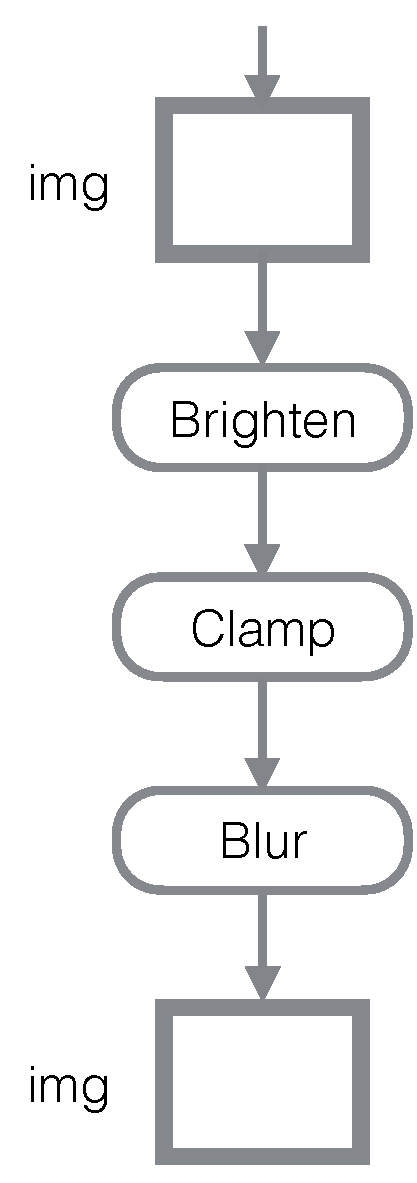
\includegraphics[scale=0.2]{./figures/motivating_example.pdf}

\end{subfigure}
\hspace*{\fill}
\begin{subfigure}{.35\textwidth}
 \begin{lstlisting}[language=C,escapechar=@]
float b1[M][3], b2[M][3], img[N][M][3]
for (i in 0..N)
 for (j in 0..M)
  for (c in 0..3)
   b1[j][c] = 1.5*img[i][j][c]@\label{fig:motivating:code1:stmt1}@
 for (j in 0..M )
  for (c in 0..3)
   b2[j][c] = clamp(b1[i][j][c], 0, 255)@\label{fig:motivating:code1:stmt2}@
 for (j in 0..M)
  for (c in 0..3)
   img[i][j][c] = (b2[j-1][c] + b2[j][c] +@\label{fig:motivating:code1:stmt3}@
                   b2[j+1][c])/3
\end{lstlisting}
\end{subfigure}
\caption{\label{fig:motivating:example} Motivating example.}
\end{figure}


%**********************************************************************************

\begin{figure}[t!]

\centering
\scriptsize

\begin{tabular}{cl}
{\textbf{\normalsize(a)}} &

\begin{lstlisting}[language=C,escapechar=@]
float b1[N][M][3], b2[N][M][3], img[N][M][3]
Parallel for (i in 0..N)
 for (j in 0..M)
  for (c in 0..3)
   b1[i][j][c] = 1.5*img[i][j][c]@\label{fig:motivating:code2:stmt1}@
 for (j in 0..M )
  for (c in 0..3)
   b2[i][j][c] = clamp(b1[i][j][c], 0, 255)@\label{fig:motivating:code2:stmt2}@
 for (j in 0..M)
  for (c in 0..3)
   img[i][j][c] = (b2[i][j-1][c] + b2[i][j][c] +@\label{fig:motivating:code2:stmt3}@
                   b2[i][j+1][c])/3
\end{lstlisting}

\\\hline

{\textbf{\normalsize(b)}} &
\begin{lstlisting}[language=C,escapechar=@]
float b1[N][M][3], b2[N][M][3], img[N][M][3]
Parallel for (i in 0..N)
 for (j in 0..M)
  for (c in 0..3)
   b1[i][j][c] = 1.5*img[i][j][c]@\label{fig:motivating:code3:stmt1}@
   b2[i][j][c] = clamp(b1[i][j][c], 0, 255)@\label{fig:motivating:code3:stmt2}@
 for (j in 0..M)
  for (c in 0..3)
   img[i][j][c] = (b2[i][j-1][c] + b2[i][j][c] +@\label{fig:motivating:code3:stmt3}@
                   b2[i][j+1][c])/3
\end{lstlisting}

\\\hline

{\textbf{\normalsize(c)}} &
\begin{lstlisting}[language=C,escapechar=@]
float b2[N][M][3], img[N][M][3]
Parallel for (i in 0..N)
 for (j in 0..M)
  for (c in 0..3)
   float t = 1.5*img[i][j][c]@\label{fig:motivating:code4:stmt1}@
   b2[i][j][c] = clamp(t, 0, 255)@\label{fig:motivating:code4:stmt2}@
 for (j in 0..M)
  for (c in 0..3)
   img[i][j][c] = (b2[i][j-1][c] + b2[i][j][c] +@\label{fig:motivating:code4:stmt3}@
                   b2[i][j+1][c])/3
\end{lstlisting}

\\\hline

{\textbf{\normalsize(d)}} & 
\begin{lstlisting}[language=C,escapechar=@]
float b2[3][N][M], img[N][M][3]
Parallel for (i in 0..N)
 for (j in 0..M)
  for (c in 0..3)
   float t = 1.5*img[i][j][c]@\label{fig:motivating:code5:stmt1}@
   b2[c][i][j] = clamp(t, 0, 255)@\label{fig:motivating:code5:stmt2}@
 for (j in 0..M)
  for (c in 0..3)
   img[i][j][c] = (b2[c][i][j-1] + b2[c][i][j] +@\label{fig:motivating:code5:stmt3}@
                   b2[c][i][j+1])/3
\end{lstlisting}

\\\hline

{\textbf{\normalsize(e)}} & 
\begin{lstlisting}[language=C,escapechar=@]
float b2[3], img[N][M][3]
Parallel for (i in 0..N)
 for (j in 0..M)
  for (c in 0..3)
   b2[0] = clamp(1.5*img[i][j-1][c], 0, 255)
   b2[1] = clamp(1.5*img[i][j][c], 0, 255)
   b2[2] = clamp(1.5*img[i][j+1][c], 0, 255)
   img[i][j][c] = (b2[0] + b2[1] + b2[2])/3
\end{lstlisting}

\\

\end{tabular}

\caption{
(a) Full expansion of b1 and b2 to allow parallelism;
(b) Loop fusion;
(c) Contraction of b1 and b2 to scalars;
(d) Transformation to AOS (Array Of Structures) for GPU execution; and
(e) Full fusion with redundant computation and contraction}
\label{fig:example-ir}

\end{figure}

In Figure~\ref{fig:motivating:example}, an obvious optimization is the parallelization of the outermost loop (over the \lstinline{i} iterator).  In order to parallelize the loop, we must first expand the two-dimensional arrays \lstinline{b1} and~\lstinline{b2} into three-dimensional arrays.  The resulting code is shown in Figure~\ref{fig:example-ir}-\codeone{}.  Another possible optimization is to fuse the loops of the blur and clamp stages.  The resulting code is shown in Figure~\ref{fig:example-ir}-\codetwo{}

If we further assume that \lstinline{img} is the only consumer of \lstinline{b1} and \lstinline{b2}, then the \lstinline{b1} array can be replaced with a scalar, as shown in Figure~\ref{fig:example-ir}-\codethree{}.  If we plan on executing on a GPU, changing from a Structure-of-Arrays (SoA) memory layout to an Array of Structures (AoS) layout may lead to better performance.  Figure~\ref{fig:example-ir}-\codefour{} shows the code after this transformation.

To maximize parallelism and data locality, we should fuse all loops of the pipeline.  Loop fusion is possible at the expense of redundant computation, as shown in Figure~\ref{fig:example-ir}-\codefive{}.  Since only 3 elements of \lstinline{b2} are computed and then immediately consumed in each iteration of the \lstinline{c} loop, we contract the array \lstinline{b2} into just three elements.

These examples demonstrate that the optimal data layout depends on how the code is scheduled, as well as knowledge about consumers of values produced by the code; that is, the data layout depends on the schedule of the program as well as producer-consumer relationships.
These examples show the need for an intermediate representation that avoids committing to a specific data layout at an early stage, since sometimes it is advantageous to perform data layout mapping only after deciding on the computation schedule and composition.
Trying different schedules and different data mappings for the same schedule also becomes easy with this separation and the search for schedule and data-layout can be automated using an auto-tuner~\cite{opentuner}.
%Furthermore, this separation allow domain specific languages to become fully architecture-independent and portable.

\subsection{Intermediate Representations}
The three intermediate representations of \framework stage the incorporation of algorithm, schedule and data layout into the final program representation.
The IR uses a mathematical representation based on the polyhedral model~\cite{feautrier_dataflow_1991,Karp:1967:OCU:321406.321418,Ancourt:1991:SPL:109625.109631,Bas04,bondhugula_effective_2010} with extensions to support non-quasi-affine\footnote{A detailed definition of quasi-affine constraints is provided in Section~\ref{qaffine}, but in general, quasi-affine expressions are linear expressions over the loop iterators and loop parameters.} iteration spaces~\cite{benabderrahmane_polyhedral_2010,pencil}.  This enables the framework to apply advanced transformations on arbitrary loop nests. A typical workflow for using \framework is illustrated in Figure~\ref{fig:overview}.  DSL compilers parse input programs and perform domain specific optimizations before translating the DSL program into Layer I of the \framework intermediate representation.  The first layer of the IR is then transformed to lower layers (Layer II and Layer III), and finally LLVM IR is generated.

\begin{figure}
 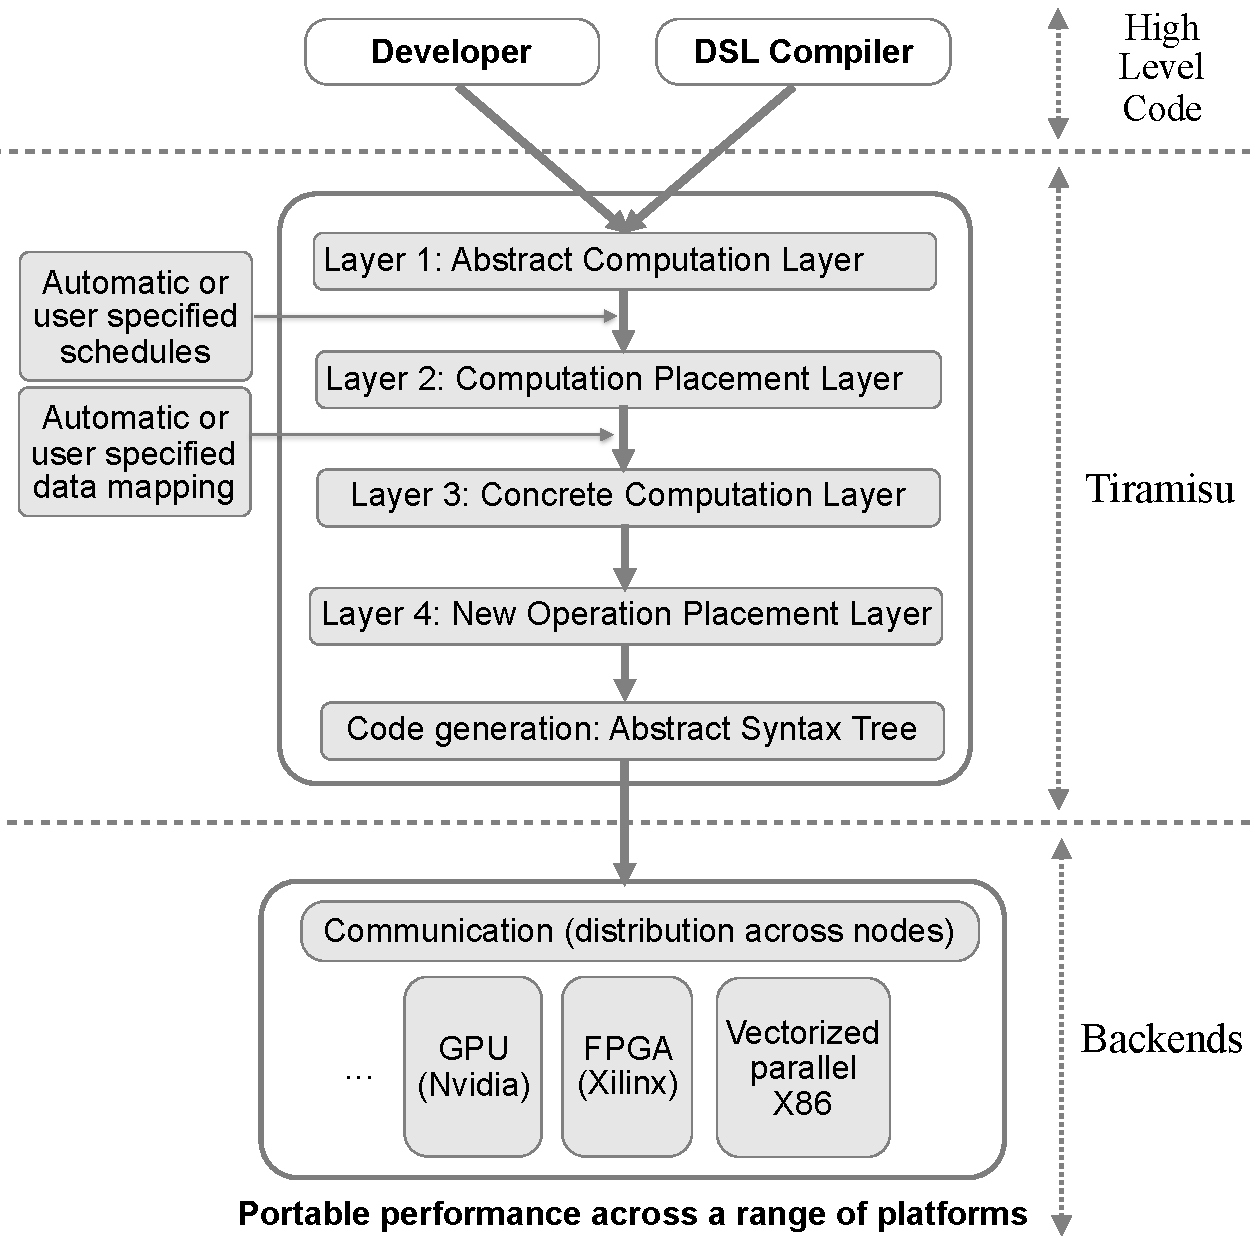
\includegraphics[scale=0.35]{./figures/fista.pdf}
 \caption{\framework overview}
 \label{fig:overview}
\end{figure}

The three layers of the \framework IR are: 
\begin{itemize}
  \item Layer I (\Layerone) specifies the computations (i.e. the algorithm) without specifying the schedule (i.e. when and where the computations occur) or how data should be stored in memory (data layout). As there is no notion of a data location, values are communicated via explicit producer-consumer relationships between the producing statement and all consuming expressions.  
  \item Layer II (\Layertwo) uses a {\it time-\processor vector} to specify when and where the computations occur, i.e. in which order and on which logical processor. This layer does not specify how intermediate values are stored in memory; this simplifies optimization passes at this layer since these passes do not need to perform complicated data-layout transformations. 
  %However, it uses a multi-dimensional time-\processor vector, that can represent many complex computation placements.
  \item Layer III (\Layerthree) makes the data layout concrete, specifying where in memory intermediate values are stored.
\end{itemize}

The separation into levels does not imply that data-layout mapping must always occur after scheduling the computation; in \framework, the user can still specify data layout before scheduling (to constrain the scheduling, for example). However, the separation ensures that the scheduling phase can safely assume no data-layout transformations are required, greatly simplifying scheduling transformations.

%\framework provides mechanisms for transforming the IR into subsequent levels.  Users specify a sequence of transformations to apply (e.g. tiling, splitting, fusion, parallelization, vectorization, or any arbitrary quasi-affine transformation), and the framework applies them and generates code but it does not provide any automatic way to decide which schedules and data layouts are valid, or which will result in the most optimal code. Such automation is beyond the scope of this paper.

While simple primitives and time-processor-vectors provide an easy path from Layer I to Layer III,   
the underlying polyhedral representation  allows the \framework to handle much more complicated iteration spaces and advanced iteration space transformations.
Transformations from iteration space in Layer I to the time-\processor space in Layer II and then the time-\processor vector to the data layout in Layer III can be expressed as quasi-affine relations. %Transformations between layers can also be performed using a non-quasi-affine transformation framework as long as such a framework can start from code in one IR layer and generate another layer of the IR.

\begin{comment}

\begin{figure}
\small

\centering\begin{lstlisting}[language=C,escapechar=@,basicstyle=\linespread{0.9}\small\ttfamily]
for (i in 0..N)
  for (j in 0..M)
    S1
    S2
\end{lstlisting}
(a) Original computation expressed as an imperative program


\begin{tabular}{c|c}
\\\hline
   \begin{tabular}{l@{\hspace{4pt}}r@{\hspace{2pt}}c@{\hspace{2pt}}c@{\hspace{2pt}}c@{\hspace{0pt}}l}
    S1: & [ & $i,$ & $j$, & $0$ & ] \\
    S2: & [ & $i$, & $j$, & 1 & ] \\
    \multicolumn{6}{c}{ (b) Sequential}
   \end{tabular}
     &  
   \begin{tabular}{l@{\hspace{4pt}}r@{\hspace{2pt}}c@{\hspace{2pt}}c@{\hspace{2pt}}c@{\hspace{0pt}}l}
    S1: & [ & $j$, & $i$, & 0 & ] \\
    S2: & [ & $j$, & $i$, & 1 & ] \\
    \multicolumn{6}{c}{ (c) Transposed}
   \end{tabular} \\\hline

    \begin{tabular}{l@{\hspace{4pt}}r@{\hspace{2pt}}c@{\hspace{2pt}}c@{\hspace{2pt}}c@{\hspace{0pt}}l}
    S1: & [ & $i$, & 0, & $j$ & ] \\
    S2: & [ & $i$, & 1, & $j$ & ] \\
    \multicolumn{6}{c}{ (d) Inner loop fission}
   \end{tabular} 
   & 
    \begin{tabular}{l@{\hspace{4pt}}r@{\hspace{2pt}}c@{\hspace{2pt}}c@{\hspace{2pt}}c@{\hspace{0pt}}l}
    S1: & [ & 0, & $i$, & $j$ & ] \\
    S2: & [ & 1, & $i$, & $j$ & ] \\
    \multicolumn{6}{c}{ (e) Outer loop fission}
   \end{tabular} \\\hline
   
    \begin{tabular}{l@{\hspace{4pt}}r@{\hspace{2pt}}c@{\hspace{2pt}}c@{\hspace{2pt}}c@{\hspace{2pt}}c@{\hspace{0pt}}l}
    S1: & [  & $i/N$, & $i\%N$, & $j$, & 0 & ] \\
    S2: & [  & $i/N$, & $i\%N$, & $j$, & 1 & ] \\
    \multicolumn{6}{c}{ (f) Loop split}
   \end{tabular} 
   &
    \begin{tabular}{l@{\hspace{4pt}}r@{\hspace{2pt}}c@{\hspace{2pt}}c@{\hspace{2pt}}c@{\hspace{2pt}}c@{\hspace{0pt}}l}
    S1: & [ & $i/N$, & $j$, & $i\%N$, & 0 & ] \\
    S2: & [ & $i/N$, & $j$, & $i\%N$, & 1 & ] \\
    \multicolumn{6}{c}{ (g) ... \& permuted}
    \end{tabular}  \\\hline
    
    \begin{tabular}{l@{\hspace{4pt}}r@{\hspace{2pt}}c@{\hspace{2pt}}c@{\hspace{2pt}}c@{\hspace{2pt}}c@{\hspace{0pt}}l}
    S1: & [ & $i\%P$ {\it (cpu)}, & $j$, & $i/P$, & 0 & ] \\
    S2: & [ & $i\%P$ {\it (cpu)}, & $j$, & $i/P$, & 1 & ] \\
    \multicolumn{6}{c}{ (h) Outer parallel }
   \end{tabular} 
   &
    \begin{tabular}{l@{\hspace{4pt}}r@{\hspace{2pt}}c@{\hspace{2pt}}c@{\hspace{2pt}}c@{\hspace{2pt}}c@{\hspace{0pt}}l}
    S1: & [ & $i$, & $j/4$, & 0, & $j\%4$ {\it (vec)} & ] \\
    S2: & [ & $i$, & $j/4$, & 1, & $j\%4$ {\it (vec)} & ] \\
    \multicolumn{6}{c}{ (i) Inner vectorized }
   \end{tabular} \\ 

\end{tabular}
 \caption{For a simple loop next with two statements, examples of different time-processor vectors leading to many possible execution arrangements. }
\label{fig:time-processor-vector}
\end{figure}

\end{comment}

%\subsection{Time-Processor Vectors}

% to map an iteration into a \processor and time order.
%The {\it time-\processor vector} in Layer II is a vector indicates the logical time of execution of computations and the processor on which they should be executed.
%Computations in Layer II are represented as {\it time-\processor vectors}.  Each one of those vectors has a name associated to it (the name of the computation). $S1[0,0,0]$, $S2[0,0,1]$, $S1[i,j,0]$ and $S2[i(cpu),j,1]$ are  examples of time-\processor vectors representing computations in Layer II.
%In general, the  time-\processor vector has two types of dimensions: time dimensions and \processor dimensions.
%The time dimensions provide the logical order of execution of the computations while the \processor dimensions indicate on which processor the computations should be executed.
%In the previous example, the first three vectors have time dimensions only, while the last vector has one space dimension.
%We use a tag to indicate that a given dimension is a \processor dimension; this tag indicates mainly the type of processor to which the computations are mapped.%: cpu, gpu, node (for a distributed system), etc.

%Assuming that we have two time-\processor vectors we want to know which vector among the two executes first, then all we need to do is to compare the two vectors lexicographically~\footnote{A \emph{time-\processor vector} $[i_1, \dots, i_k, \dots, i_n]$ lexicographically precedes another time-\processor vector $[i_1', \dots, i_k', \dots, i_n']$ if and only if $\exists k \in \mathbb{N}$ such that $i_1 = i_1' \wedge i_2 = i_2' \wedge \dots \wedge i_k < i_k'$}.
%In the example, $S1[0,0,0]$ precedes $S2[0,0,1]$ lexicographically, so $S1[0,0,0]$ is scheduled to be executed before $S2[0,0,1]$.
%The ability to add dimensions and reorder them freely enables the expression of multiple possible mappings from the original iteration space of the computations to complex execution scenarios.
%Figure~\ref{fig:time-processor-vector} provides examples of different optimizations for a simple algorithm and shows the  time-\processor vectors used to express those optimizations.
%Each of the dimensions of the vector can be an indexed variable, distributing the computation over that dimension or a constant providing a lexical ordering between statements. 
%The algorithms will be using a custom intermediate representation within each DSL, however, we use a classical imperative language representation to describe them in this paper.
%A value can be annotated by a processor type, indicating where that computation will be placed, and indicating that dimension will be run in parallel.





\subsection{Why is an Extended Polyhedral Representation Required}

Example that requires shifting for fusion,

\begin{figure}[ht]

\begin{lstlisting}[language=C,escapechar=@]
/* Loop 1: Ring Blur Filter */
for (i = 1; i < length - 1; i++)
 for (j = 1; i < width - 1; j++)
  Ring[i][j] = (Img[i-1][j-1] + Img[i-1][j] + Img[i-1][j+1]+
                Img[i][j-1] + Img[i][j+1]+
                Img[i+1][j-1]+Img[i+1][j]+ Img[i+1][j+1])/8;

/* Loop 2: Roberts Edge Detection Filter */
for (i = 1; i < length - 2; i++)
 for (j = 2; i < width - 1; j++)
  Img[i][j] = abs(Ring[i][j] - Ring[i+1][j-1])+ abs(Ring[i+1][j] - Ring[i][j-1]);

\end{lstlisting}

\caption{\label{fig:motivating:example2} Second motivating example.}
\end{figure}



\subsection{Three-Layer IR Example}
Figure~\ref{fig:example-ir} shows the code for each one of the optimizations discussed in the previous section along with its three-level IR representation (Layer I, II and III) on the right. A more formal definition of each IR layer and inter-level transformations is presented in Sections~\ref{sec:ir}--\ref{sec:compilation}.  
The Layer I representation, provided by the high-level DSL compiler, is common between all the code variants, regardless of how they are optimized. Porting the code to a new machine does not require changing the algorithm; only the schedule and data mapping need to be changed.
The Layer II representation is the same for code variants that have the same schedule but only differ in the data mapping; this is the case for Figures~\ref{fig:example-ir}-\codetwo{} and~\ref{fig:example-ir}-\codethree{} as scalarization does not require changes to the schedule.

Each line in Layer I of Figure~\ref{fig:example-ir}-\codeone{} (right side in the figure) corresponds to a statement in the original algorithm (left side of the figure): for example, the second line of Layer I represents the line~\ref{fig:motivating:code1:stmt1} in Figure~\ref{fig:example-ir}-\codeone{}.
The first part of that line, which is $\{b_1\ (i, j): 0\leq i < N \wedge 0\leq j < M\}$, represents the iteration space of the statement, while the second part, $a(0)*f_1(i, j)$, is an expression that represents what is computed (note that we represent the scalar $a$ as an array of length 1).
The iteration space is the set of tuples $(i,j)$ such that $0\leq i < N \wedge 0\leq j < M$, and is used to define the set of computations $b_1(i,j)$.  Each computation $b_1(i,j)$ computes the expression $a(0)*f_1(i,j)$.  The set of integer tuples is compactly described by a set of constraints (quasi-affine constraints over the loop iterators and symbolic constants; see Section~\ref{qaffine} for details).  We use $b_1$ as the collective name of the static producer and $b_1(i,j)$ denotes a particular dynamic instance of that producer.  It refers to the value produced by the $(i,j)$ iteration.

%The key idea of this level is to define the computations independent of memory locations and intermediate storage, so this level does not say anything about the order of computations or their storage.  For example, the last line in Figure~\ref{fig:example-ir}, defining the computation of $avg$, is the same regardless of which of the optimized implementations in Figures~\ref{fig:motivating:code1}--\ref{fig:motivating:code4} we represent. 

The computations in Layer I are not ordered.  The order in which they are declared does not have any effect on their actual order of execution.  The actual order of execution is specified in Layer II.
%The order imposed by the producer-consumer relationships is not explicitly represented in the IR layers, but it can be easily computed using polyhedral array data flow analysis~\cite{feautrier_dataflow_1991}. Dependence analysis in Layer I is effective because of the absence of aliasing problems given that the IR does not have any notion of pointers and given that every computation is only defined once.

%For example, whether the computations $out(i,j)$ are stored in a contracted array, in a scalar or whether they are duplicated for execution on different CPUs, the consumer does not need to change.  Only the data mapping (in layer III) needs to be modified depending on the data layout chosen.




An example of the Layer II representation is shown on the right side of Figure~\ref{fig:example-ir}-\codeone{}.
The main difference between Layer I and II is that computations in Layer II are ordered using a time-processor vector while computations in Layer I are not.  The set $\{b_1[1, i (cpu, virtual), 0, j]:  0\leq i < N \wedge 0\leq j < M\}$, in the example, is an ordered set of computations where the time-processor vector $[1, i (cpu, virtual), 0, j]$ orders the computation and maps it to the $i$th virtual CPU.  The tag \emph{(cpu)} for the $i$ dimension indicates that this dimension is a \processor dimension and that each $i$th iteration is mapped to the $i$th CPU. Adding the tag \emph{(virtual)} indicates that the CPU to which the computations are mapped is a virtual CPU; a virtual CPU is mapped by the runtime to any physical CPU during execution.  To identify the logical order of execution between the computations mapped to the same processor, we project out (remove) the \processor{} dimensions and keep only the time dimensions of the time-processor vector ($[1, 0, j]$ in the previous example); then we compare these computations based on their lexicographical order~\footnote{Although the computations have different names, when comparing them we ignore those names and consider that they are all a part of the same time-\processor{} space.}.
%This is denoted as follows $$[i_1, i_2, \dots, i_k, \dots, i_n] \ll [i_1', i_2', \dots, i_k', \dots, i_n']$$.

%Figure~\ref{} shows how we can represent the order of execution of the statements in Figure~\ref{} and their placement using a \emph{time-\processor } vector.

%  A dimension can be a dynamic dimension (usually a loop iterator or a linear combination of the loop iterators and parameters), and can also be a constant (usually used to specify the order between statements that have the same iteration space but only differ in their order within  the statements, . Iteration variables normally provide sequential execution or can be annotated with a virtual processor, providing parallel execution. 

%Although, all the computations in layer II are a part of the same space, which is the time-\processor space, we use different names for the different computations.  Such names in layer II are a syntactic sugar used for convenience only and are ignored when comparing the lexicographical order of computations.

%The transformation of layer I into layer II can be done automatically using an affine schedule (relation) that maps the computations from the iteration space to the time-\processor space.  It can also be done using a non-affine transformation technique as long as the technique guarantees that the generated layer II satisfies some constraints that we specify in Section~\ref{layer2}.

%In the example, Figures~\ref{fig:example-ir}-\codetwo{} and~\ref{fig:example-ir}-\codethree{} share the same Layer II representation.  They only differ in their Layer III representation.

Layer III of Figure~\ref{fig:example-ir}-\codeone{} is the last layer of the \framework IR.  At this layer, we keep the same Layer II representation and add the mapping to data-layout (memory buffers and scalars are also declared in this layer).
This layer indicates where each computation is stored in memory.  In the example, the data mapping $\{b_1[1, i (cpu, virtual), 0, j] \rightarrow {buf}_{b1}[i,j]:  0\leq i < N \wedge 0\leq j < M\}$ indicates that the result of the computation $b_1[1, i (cpu, virtual), 0, j]$ is stored in the array element ${buf}_{b1}[i,j]$.
%(in the contracted array $buf_{b1}[N,3]$).
The data mapping in general is a quasi-affine relation that maps a computation from the time-\processor space to a buffer element (scalars are one element buffers).  \framework allows the expression of all the data-layout mappings that can be expressed as quasi-affine relations (examples provided in Section~\ref{layer3}).
For brevity, the declaration of buffers, their types, their allocation (including when and where they are allocated), are all omitted from the example, but such information must be specified for correct code generation.

Here is another example of data layout mapping: if we want to map the $b_1$ and $b_2$ computations of Figure~\ref{fig:example-ir}-\codefour{} to an array-of-structures, it is sufficient to provide the following mapping to an array $buf_b[N, 2, \boldsymbol{2}]$ where the innermost dimension of the array (in bold) is used to represent a tuple index, which is equivalent to a slot in a structure:

\noindent $\{b_1[1, i (cpu, virtual), j, 0, k] \rightarrow buf_b[i, k, 0]:  0\leq i < N \wedge 0\leq j < M \wedge 0\leq k < 2\}$ \\
$\{b_2[1, i (cpu, virtual), j, 1, k] \rightarrow buf_b[i, k, 1]:  0\leq i < N \wedge 0\leq j < M \wedge 0\leq k< 2\}$ \\

\subsection{Scope of the Intermediate Representation}

The \framework intermediate representation is designed to be used as an IR for DSLs that logically operate over dense data using loop nests and sequences of statements.  In general, this is the case for DSLs in fields such as image processing, dense linear algebra, stencils, etc.
%The schedule and data mappings are either derived automatically or are specified by the user at the DSL language level (as in Halide~\cite{halide_12} for example).
We assume that function calls are inlined and that all iteration spaces are quasi-affine.  %The framework can represent arbitrary iteration spaces (quasi-affine and non-quasi-affine iteration spaces including while loops, loop nests with non-quasi-affine conditionals, loop nests with non-quasi-affine loop bounds, etc.).%  It can automatically transform layer I into layer II if the schedule (transformation relation) is quasi-affine; but allows the user can perform some non-quasi-affine transformations from layer I to layer II.  The framework can represent all types of data-mapping that can be expressed as quasi-affine relations.

In the following section, we provide more details about the formalism that we use to represent integer sets and maps (relations between sets).